\section*{Game Description}
The game that is used in this test is a game that has been developed as part of a 7th medialogy semester project. Therefore it is still in development. The current version on the prototype fulfill its purpose for this test. Additional features, if any, would be welcomed but is not expected to have any significant influence on the test results.

\subsection*{Tablet Game Application with a Tangible Widget}
The game is developed in Unity and is made for tablets. This is done with the intention of exploring unconventional methods for interacting with games on a tablet. For this purpose, as part of the semester project, a tangible widget, which can be seen in Figure \#, has also been produced. The tangible widget touches the tablet screen with two points, and through nails and conductive copper tape these points are registered as touch input. The center between the two touch input is computed, which is basically the user input. In this center the software computes a coloured light, which can be perceived through the light conductive material.  

The game itself is designed with the purpose of measuring a user accuracy over time in a game scenario to see if using the widget can improve the performance. Therefore, the user task is to trace a pixel thin line using the tangible widget. Two circles are displayed, starting circle is green the ending is red. The two circles are then connected by this pixel thin line. The line will only be displayed for a short period of time right when each level starts, then it fades away. The user uses the tangible widget to trace the line as accurately as possible. The help they receive to complete the given task is a light feedback ranging from green to yellow to red. When the line is being traced accurately the light is green, when they are slightly off it goes to yellow, and when the user gets too far from the line it is red. The color changes happens gradually with a ramp and does not just switch between the three colors. 

\begin{figure}[!h]

\includegraphics[width=0.85\textwidth]{img/lights}
\caption{The widget showing the three different states of light. Green on the line, Yellow slightly off, red far off.}
\end{figure}

\subsection*{Tutorial}
When the game is first started, the user is presented with a tutorial that explains the interaction with the widget on the tablet, and how to understand the light feedback. Furthermore, before the user is presented with one of the actual game levels, they get to play a level with the line they have to trace as being visible.

\begin{figure}[!h]
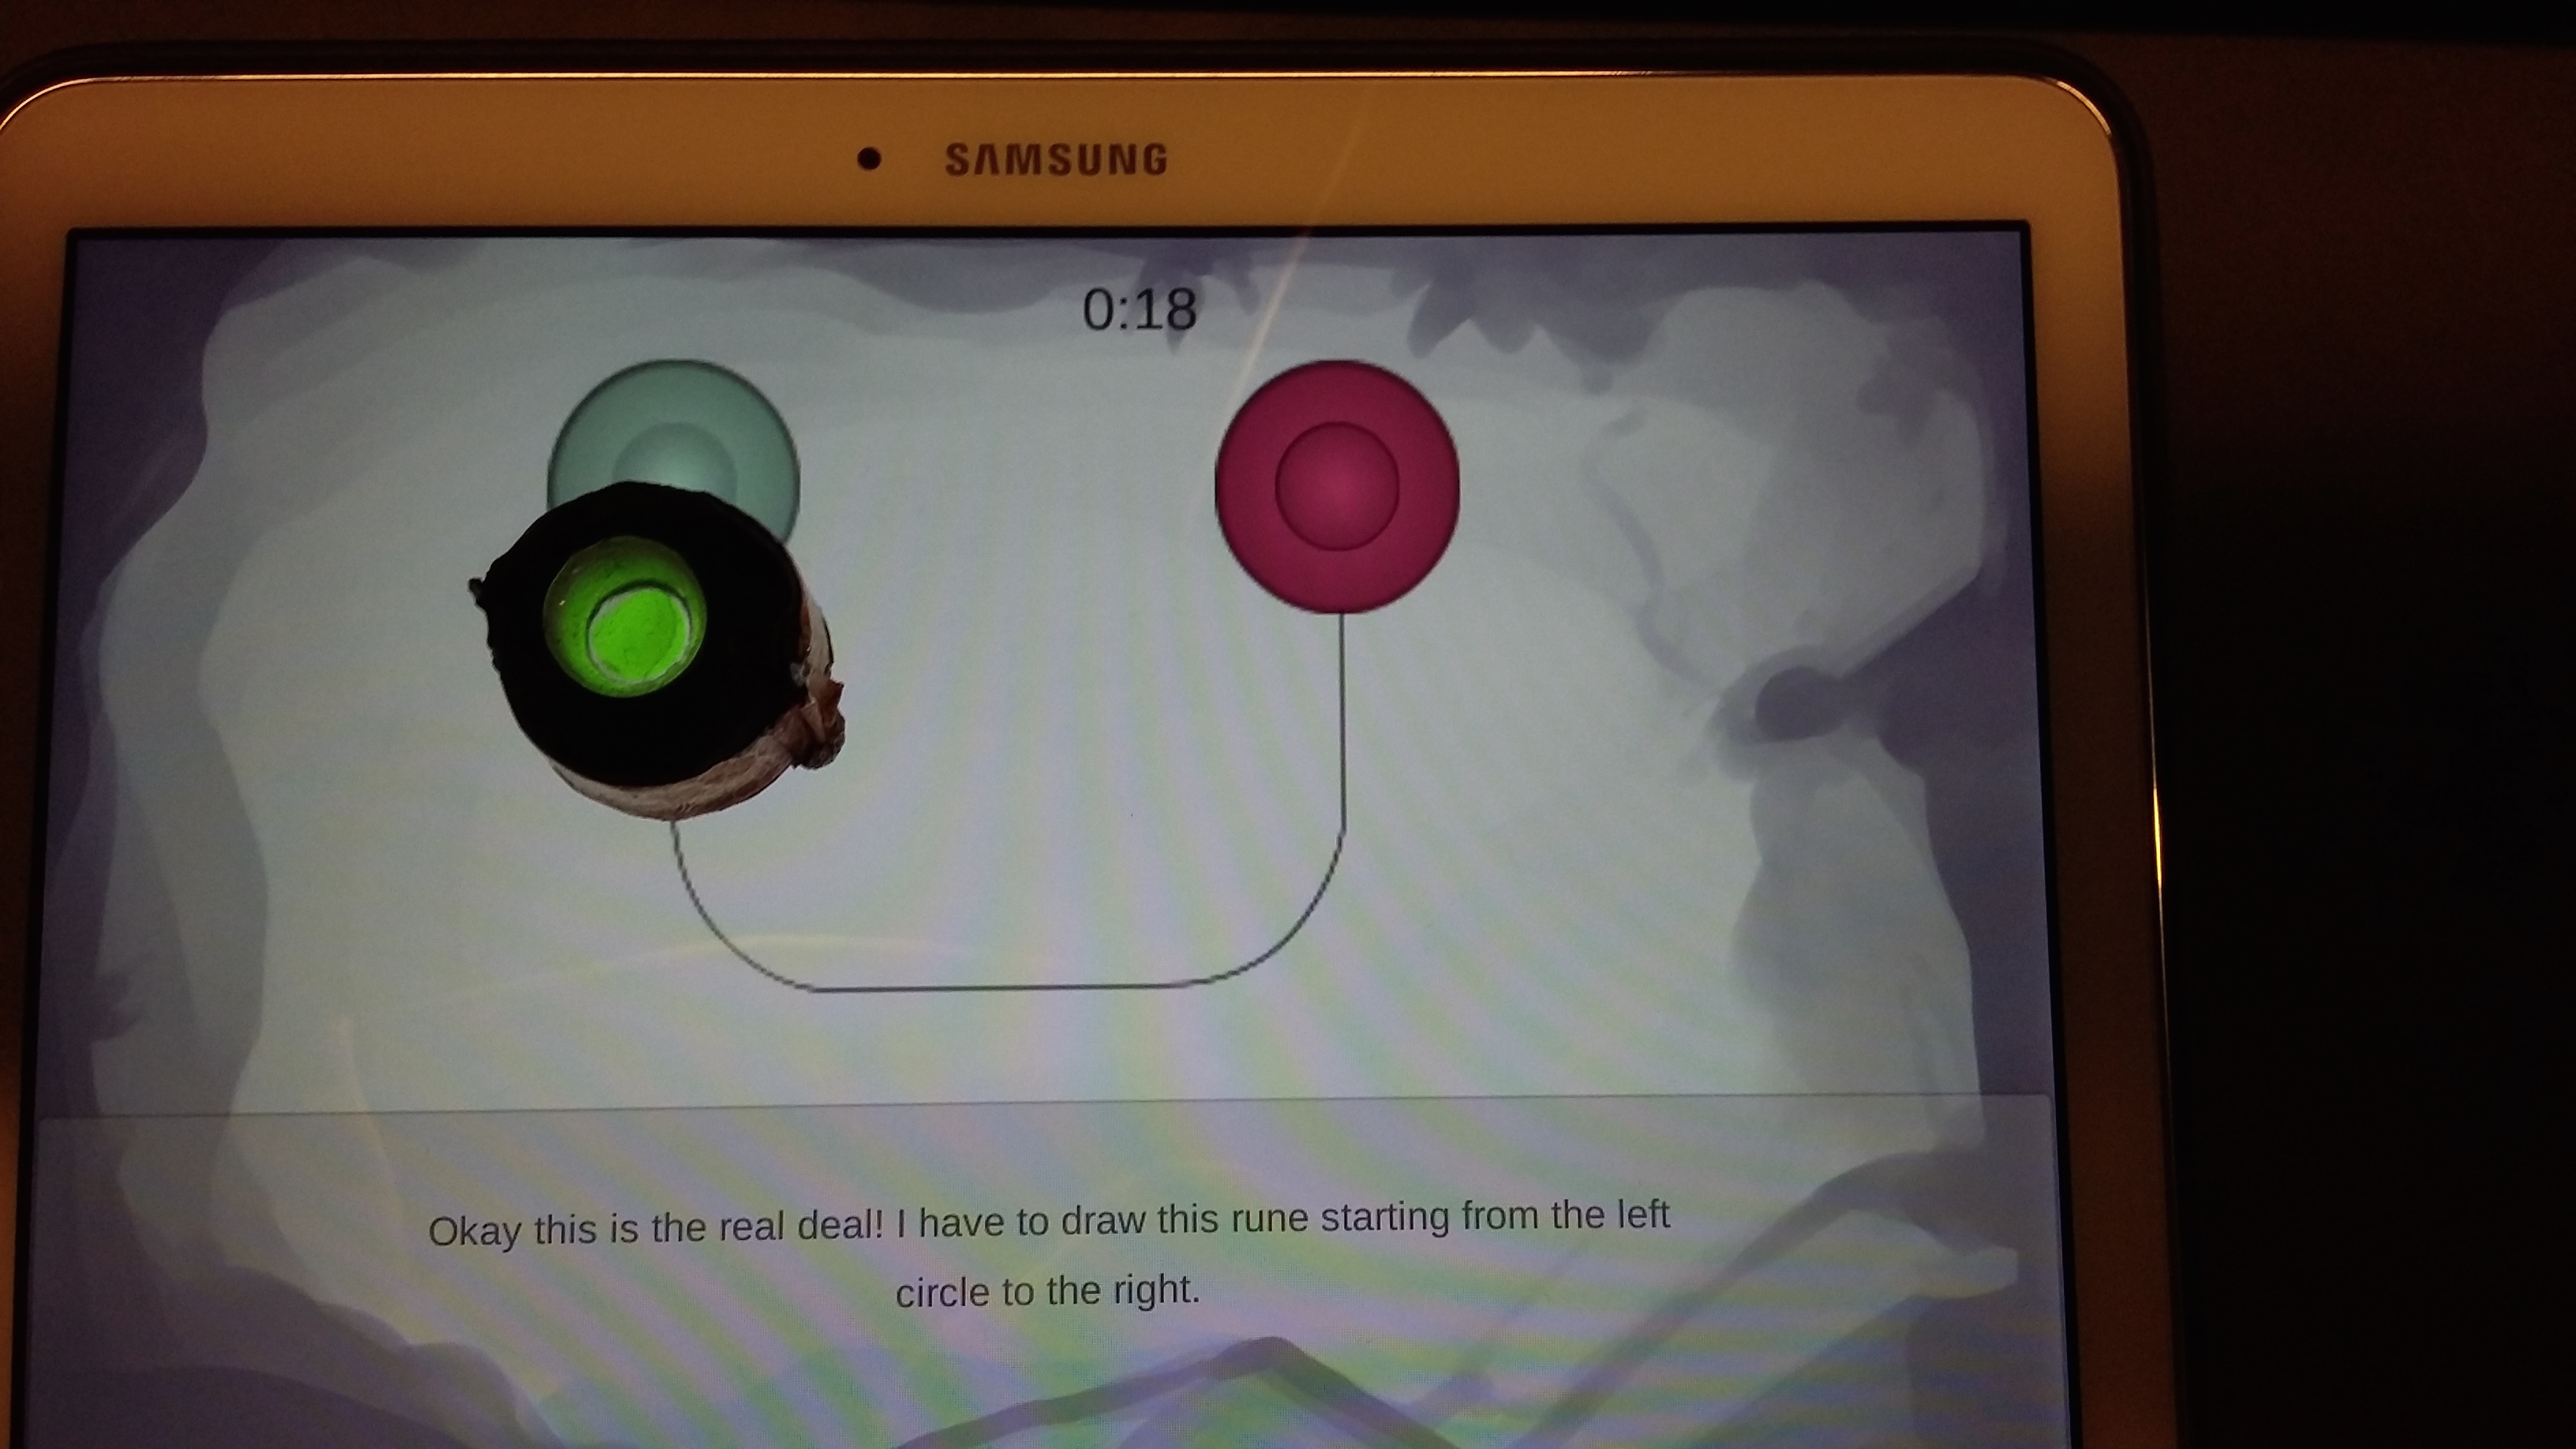
\includegraphics[width=0.85\textwidth]{img/tut}
\caption{Tutorial level with the line visible and with widget show on the line with green light coming through.}
\end{figure}

\subsection*{Level Design}
For each level there is a timer centred at the top of the screen. For this test the game has been modified so that the level will only end when the timer runs out. The user can be as accurate within the given timeframe as possible, e.g. by retracing the line or by jumping to specific parts of the line, if they wish to. They can even start back-tracing the line during an attempt to trace the line. In the original game design, however, the level would have ended upon reaching the red circle at the end of the line.

When the user completes a level their final score will displayed in a box on the middle of the screen. The score will be displayed as a number of cat heads as a score from 1-5. This value is arbitrary and the user unaware of exactly what the thresholds for each head is. Hence, they get an accuracy score in percentage where they can see exactly how many percentage of the line they managed to hit. 

\begin{figure}[!h]
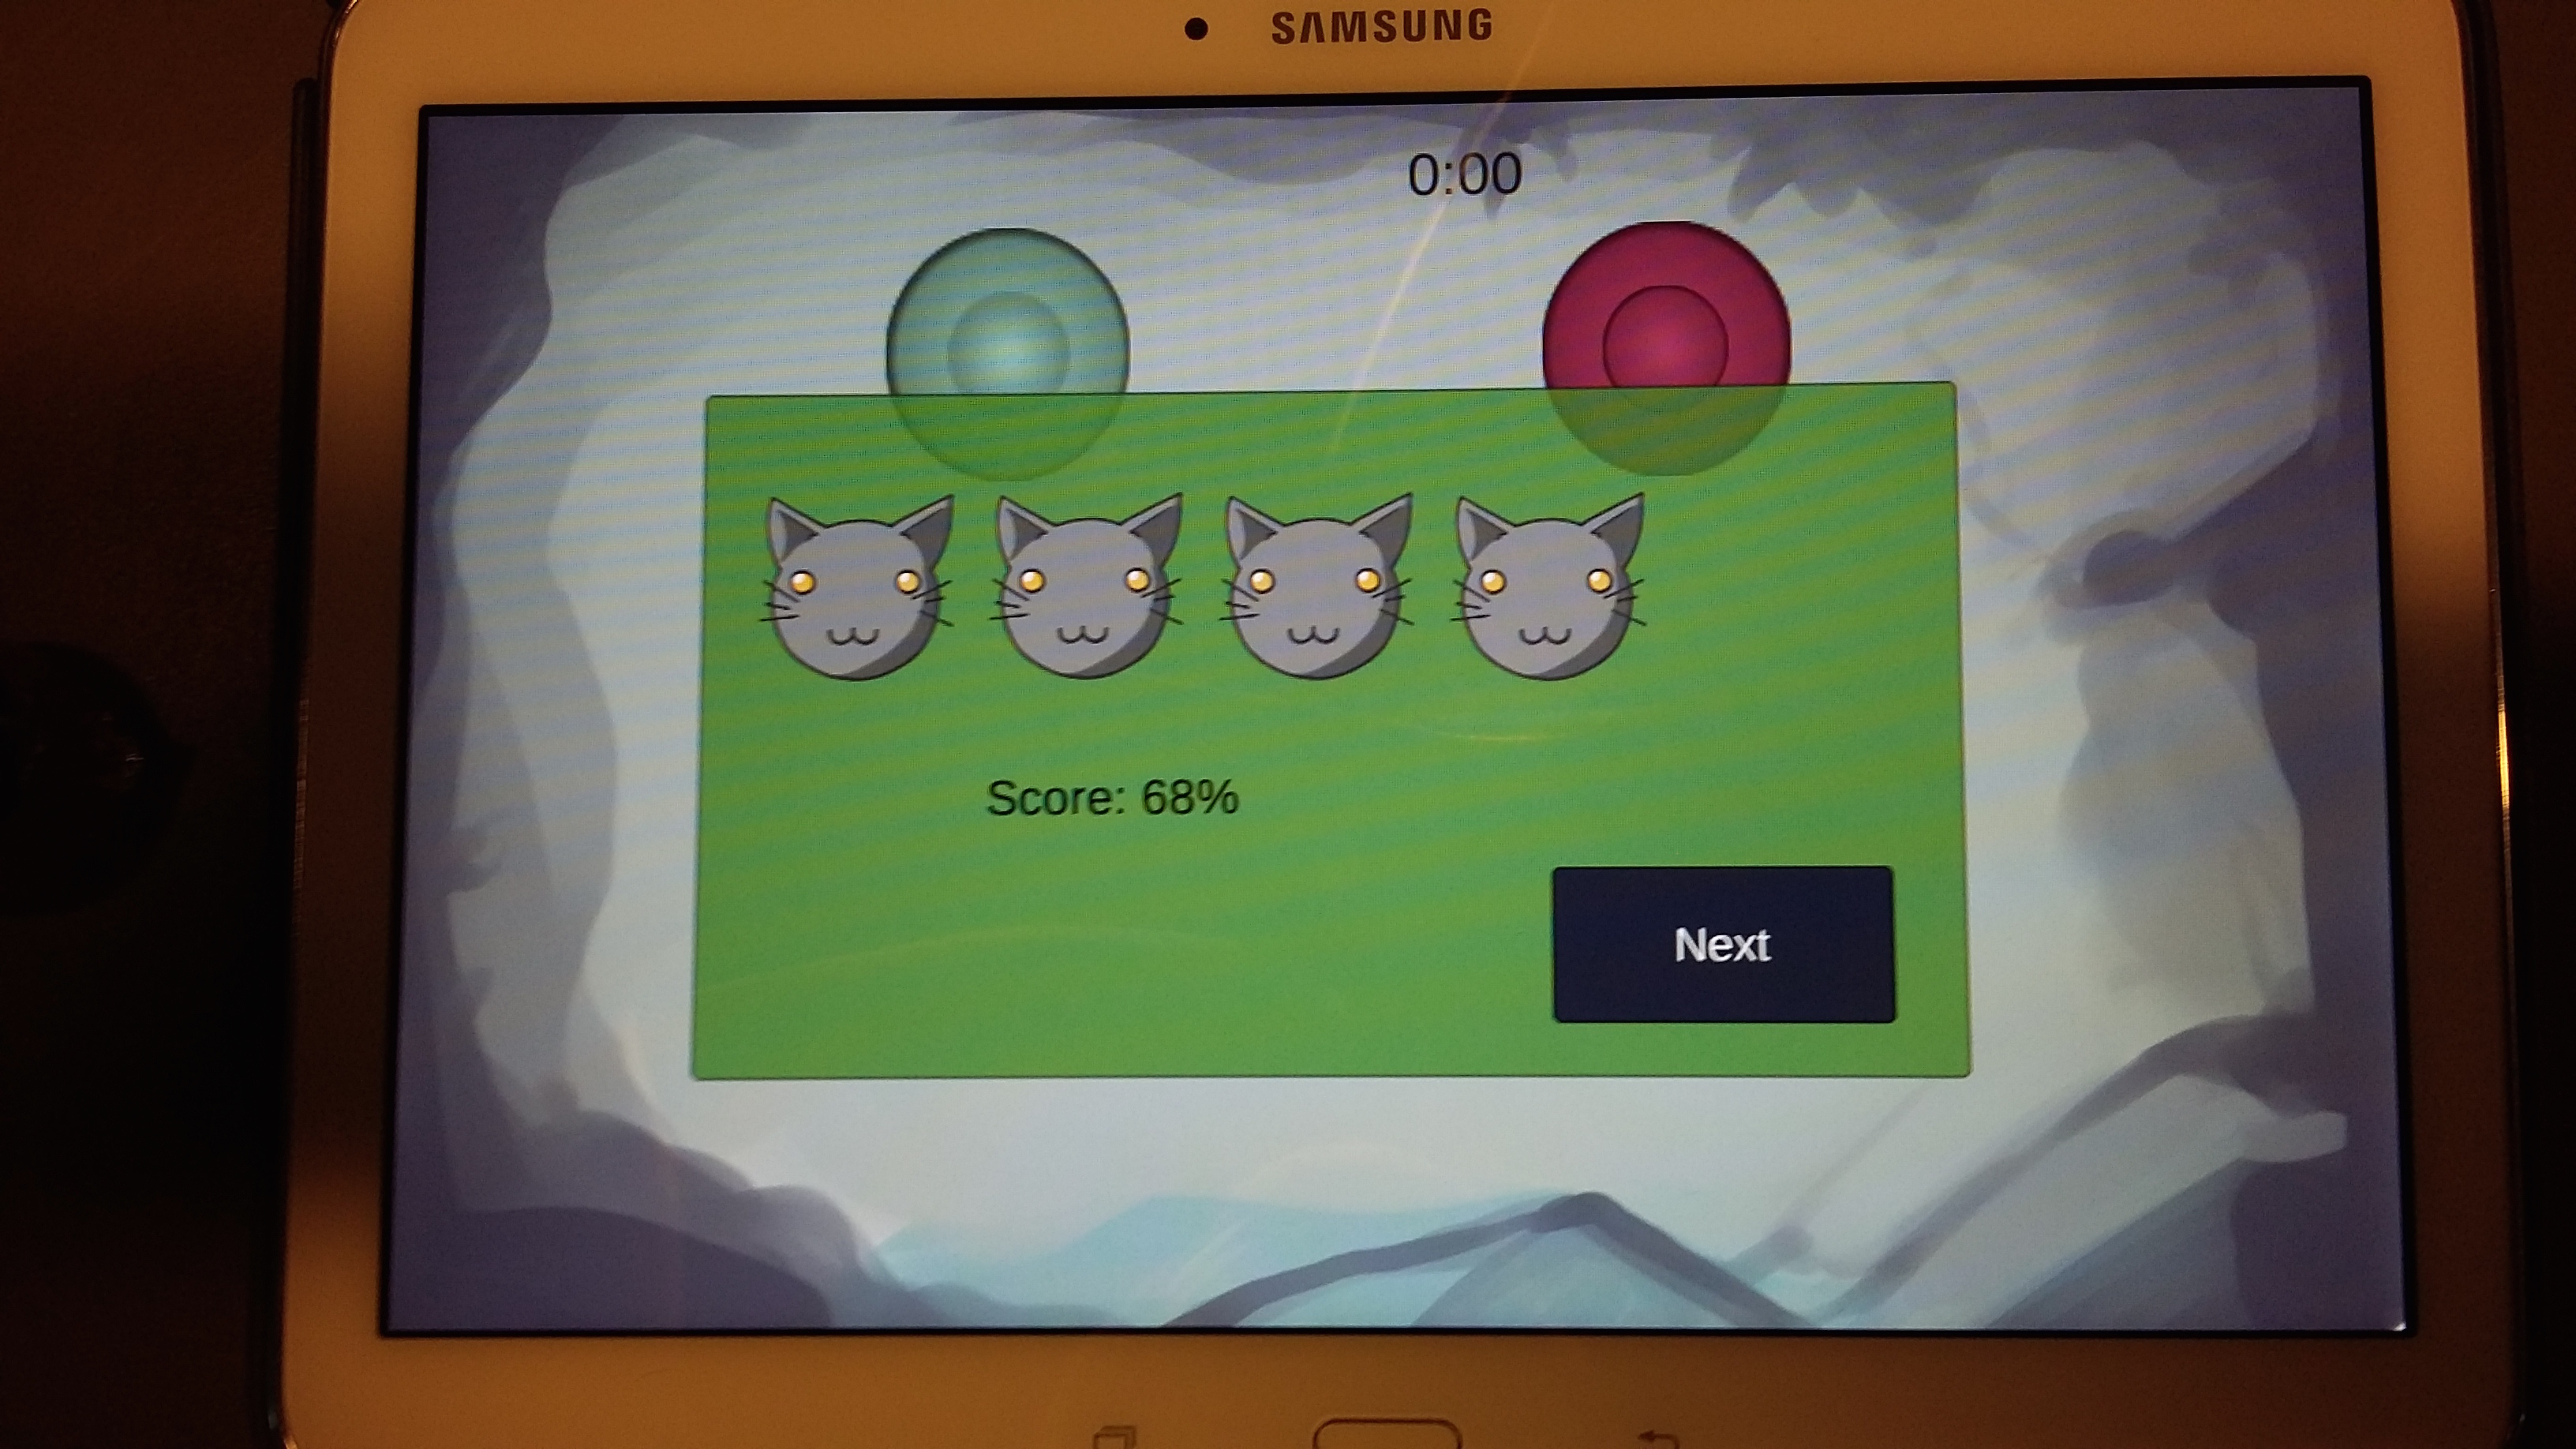
\includegraphics[width=0.85\textwidth]{img/points}
\caption{Here the user achieve the grade 4 out of 5, displayed in the form of cats, moreover the user hit 68\% of the line and can now press next to continue to the next level.}
\end{figure}
For the purpose of this experiment the game has been modified to be played by the first subject and continued by the second one. The game loops through the tutorial and then three levels of the game for both subjects. In the second playthrough the third and last level has been modified as well, so that the light feedback for tracing the line stops working halfway through the level. Initially it will be displayed as being the full line before it fades away, but the user will not be able to trace the line for more than half of the original length. 